\documentclass[12pt, a4paper]{article} %determina o tamanho da fonte, o tipo de papel e o tipo de documento.

\setlength{\parindent}{1.0 cm} %tamanho do espaço para começar o parágrafo.
\setlength{\parskip}{0.5cm} %tamanho do espaço entre os parágrafos.

%Aqui ficam os pacotes utilizados para formatação do documento de modo geral:

\usepackage[utf8]{inputenc} 
\usepackage{indentfirst} %Coloca espaços nos inícios de parágrafos automaticamente. 
\usepackage[brazilian]{babel} %
\usepackage{amsmath}
\usepackage[hmargin=3cm, vmargin=2.5cm, bmargin=2.5cm]{geometry}
\usepackage{multicol}
\usepackage{graphicx} %para poder inserir imagens
\usepackage{subfig}
\usepackage{booktabs} 
\usepackage{hyperref} %para poder adicionar links e hiperlinks
\usepackage{float} %para poder posicionar as imagens
\usepackage{subfig} %para colocar duas imagens juntas

\usepackage{listings} %para poder incluir códigos
\usepackage{xcolor}
\definecolor{codegreen}{rgb}{0,0.6,0}
\definecolor{codegray}{rgb}{0.5,0.5,0.5}
\definecolor{codepurple}{rgb}{0.58,0,0.82}
\definecolor{backcolour}{rgb}{0.95,0.95,0.92}
\lstdefinestyle{mystyle}{
    backgroundcolor=\color{backcolour},   
    commentstyle=\color{codegreen},
    keywordstyle=\color{magenta},
    numberstyle=\tiny\color{codegray},
    stringstyle=\color{codepurple},
    basicstyle=\ttfamily\footnotesize,
    breakatwhitespace=false,         
    breaklines=true,                 
    captionpos=b,                    
    keepspaces=true,                 
    numbers=left,                    
    numbersep=5pt,                  
    showspaces=false,                
    showstringspaces=false,
    showtabs=false,                  
    tabsize=2,
    morecomment={l}[!],
    language=[77]Fortran,
}
\lstset{style=mystyle}

\begin{document} %começa alguma coisa,neste caso, o documento, sempre importante lembrar de colocar o \end{} para não dar erro 
	
	\begin{titlepage}
		\begin{center}
\Huge{Universidade de São Paulo}\\
\large{Instituto de Física de São Carlos}\\
\vspace{20pt}
\vspace{200pt}
\textbf{Lista 4}\\
\vspace{8cm}
		\end{center}

\begin{flushleft}
\begin{tabbing}
Pedro Calligaris Delbem 5255417\\
\end{tabbing}
\vspace{0.5cm}
Professor: Attilio Cucchieri\\		
		\end{flushleft}
	
		\begin{center}
			\vspace{\fill}
	Maio de 2025	
		\end{center}
	\end{titlepage}

%####################################################################### SUMÁRIO
	\tableofcontents 
	\thispagestyle{empty}
	\newpage
%#########################################################################

\section{Matrix Operations}

    \subsection{Exerc\'icio 1}

        Tarefa: Calcule todos os autovalores da matriz sim\'etrica e tridiagonal $A$, definida por:
        \begin{equation*}
            A_{mm} = -2, \quad A_{m,m-1} = A_{m-1,m} = 1
        \end{equation*}

        a qual est\'a relacionada \`a discretiza\c{c}\~ao da derivada segunda em uma dimens\~ao:
        \begin{equation*}
            f''(x) \approx \frac{f(x + h) - 2f(x) + f(x - h)}{h^2}.
        \end{equation*}
        
        Use as seguintes rela\c{c}\~oes de recorr\^encia para o polin\^omio caracter\'istico $P_n(\lambda) = \det(A - \lambda I)$:
        \begin{align*}
        P_1(\lambda) &= A_{11} - \lambda, \\
        P_2(\lambda) &= (A_{22} - \lambda) P_1(\lambda) - A_{21} A_{12}, \\
        P_3(\lambda) &= (A_{33} - \lambda) P_2(\lambda) - A_{32} A_{23} P_1(\lambda), \\
        &\vdots \\
        P_m(\lambda) &= (A_{mm} - \lambda) P_{m-1}(\lambda) - A_{m,m-1} A_{m-1,m} P_{m-2}(\lambda), \\
        &\vdots \\
        P_n(\lambda) &= (A_{nn} - \lambda) P_{n-1}(\lambda) - A_{n,n-1} A_{n-1,n} P_{n-2}(\lambda).
        \end{align*}
        
        Use o m\'etodo de Newton-Raphson para calcular numericamente as ra\'izes de $P_n(\lambda)$, ou seja, os autovalores da matriz $A$.
        
        \medskip
        
        \noindent \textbf{Sugest\~ao:} escreva uma rela\c{c}\~ao de recorr\^encia tamb\'em para as derivadas primeira e segunda, em rela\c{c}\~ao \`a vari\'avel $\lambda$, das fun\c{c}\~oes $P_m(\lambda)$. Considere o caso $n \times n$, onde $n$ \'e uma entrada (input) do c\'odigo.
        
        \medskip
        
        Compare os resultados num\'ericos com o resultado exato:
        \begin{equation*}
            \lambda_m = -4 \sin^2\left( \frac{m\pi}{2(n + 1)} \right), \quad m = 1, 2, \ldots, n.
        \end{equation*}
        
        \medskip
        
        \noindent \textbf{Sugest\~ao:} use as desigualdades
        \begin{equation*}
            \max_{j = 1, \ldots, n} \left( A_{jj} + \sum_{k \ne j} |A_{jk}| \right) \geq \lambda_m \geq \min_{j = 1, \ldots, n} \left( A_{jj} - \sum_{k \ne j} |A_{jk}| \right)
        \end{equation*}
        para organizar a busca inicial das ra\'izes de $P_n(\lambda)$.

        Derivando a rela\c{c}\~ao de recorr\^encia com rela\c{c}\~ao a lambda, obtemos:
        \begin{equation*}
            P'_m(\lambda) = (A_{mm} - \lambda) P'_{m-1}(\lambda) - A_{m,m-1} A_{m-1,m} P'_{m-2}(\lambda) - P_{m-1}(\lambda)
        \end{equation*}

        Para determinar o chute inicial do Newton-Raphson, temos:
        \begin{align*}
            A_{jj} &= -2, \\
            \sum_{k \ne j} |A_{jk}| &= |A_{j, j-1}| + |A_{j, j+1}| = 1 + 1 = 2, \quad \text{para } j = 2, \ldots, n-1, \\
            \sum_{k \ne j} |A_{jk}| &= 1, \quad \text{para } j = 1 \text{ ou } j = n, \\
        \end{align*}

        E, utilizando a desigualde dada, temos:
        \begin{equation*}
            -4 \geq \lambda_{\text{máx}} \geq 0
        \end{equation*}

        Logo, \'e razoável começar com o chute inicial entre 0 e -4.

        O c\'odigo foi compilado com o comando:

    gfortran L4-5255417-ex-1.f90 -Wall -Wextra -pedantic -ffree-form -o L4-5255417-ex-1.exe  

        Resultados:

        Testou-se os seguintes casos:
        \begin{figure}[H]
            \centering
            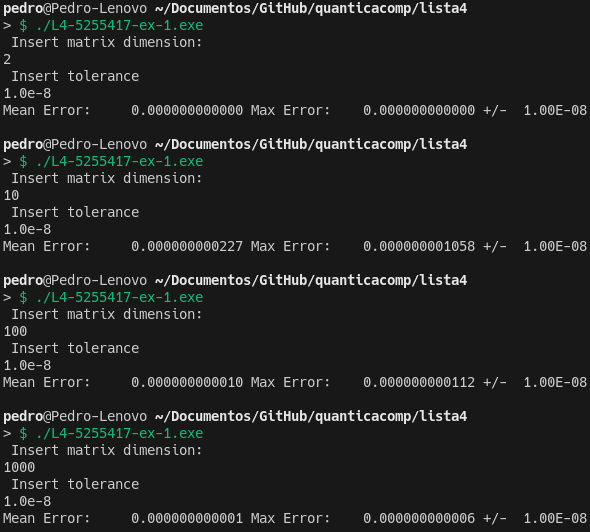
\includegraphics[width=0.4\textwidth]{../images/ex1-input.png}
            \caption{Dimens\~ao da Matriz = 1000}
        \end{figure}

        Percebe-se que a diferen\c{c}a - tanto m\'edia quanto para o maior caso - se manteve dentro da toler\^ancia em todos os casos mostrando a efici\^ancia do m\'etodo empregado.

    \subsection{Exerc\'icio 2}

        Tarefa: Considere a mesma matriz $A$ do exerc\'icio anterior e o vetor $\vec{d}$ com elementos $d_i = \delta_{i,j}$, onde $j$ \'e escolhido aleatoriamente entre os valores $1, 2, \dots, n$. Deseja-se resolver numericamente o sistema de equa\c{c}\~oes lineares $A \vec{x} = \vec{d}$, utilizando o \textbf{algoritmo de Thomas}, espec\'ifico para matrizes tridiagonais.

        O algoritmo consiste em duas fases: uma substitui\c{c}\~ao direta modificada para calcular coeficientes intermedi\'arios $d'_m$ e $c'_m$, e uma substitui\c{c}\~ao retroativa para obter a solu\c{c}\~ao final $\vec{x}$. Abaixo est\~ao as f\'ormulas utilizadas:
        
        \begin{align*}
        d'_1 &= \frac{d_1}{b_1}, &
        c'_1 &= \frac{c_1}{b_1}, \\
        d'_m &= \frac{d_m - a_m d'_{m-1}}{b_m - a_m c'_{m-1}}, &
        c'_m &= \frac{c_m}{b_m - a_m c'_{m-1}}, \quad \text{para } m = 2, 3, \dots, n-1, \\
        d'_n &= \frac{d_n - a_n d'_{n-1}}{b_n - a_n c'_{n-1}}.
        \end{align*}
        
        A solu\c{c}\~ao $\vec{x}$ \'e ent\~ao obtida pela substitui\c{c}\~ao retroativa:
        
        \begin{align*}
        x_n &= d'_n, \\
        x_m &= d'_m - c'_m x_{m+1}, \quad \text{para } m = n-1, n-2, \dots, 1.
        \end{align*}
        
        Considere o caso de uma matriz tridiagonal de dimens\~ao $n \times n$, com $n$ sendo um input do c\'odigo. Ap\'os resolver o sistema, verifique a solu\c{c}\~ao calculando o vetor res\'iduo:
        
        \[
        \vec{r} = A\vec{x} - \vec{d}.
        \]
        
        Esse vetor deve ser pr\'oximo de zero (em norma) se a solu\c{c}\~ao num\'erica estiver correta.        

        O c\'odigo foi compilado com o comando:
        \begin{verbatim}
            gfortran L4-5255417-ex-2.f90 -Wall -Wextra -pedantic -ffree-form -o L4-5255417-ex-2.exe  
        \end{verbatim}

        Resultados:

        Testou-se os seguintes casos:
        \begin{figure}[H]
            \centering
            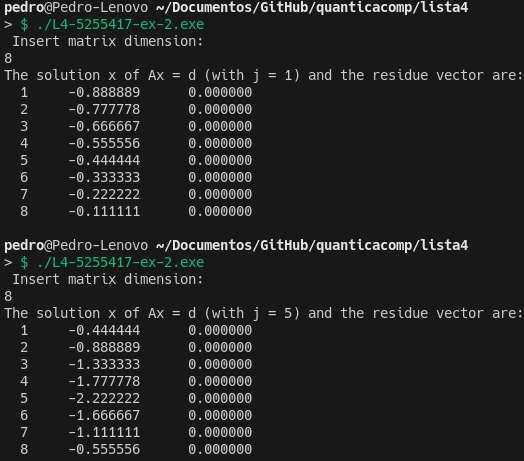
\includegraphics[width=0.8\textwidth]{../images/ex2-results-8.png}
            \caption{Testes para matriz de dimensão 8}
        \end{figure}
        \begin{figure}[H]
            \centering
            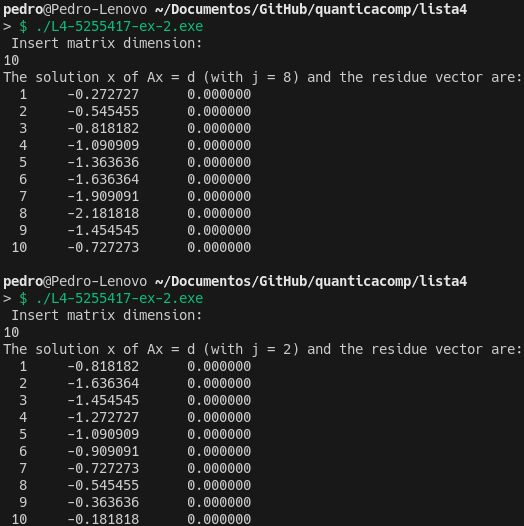
\includegraphics[width=0.8\textwidth]{../images/ex2-results-10.png}
            \caption{Testes para matriz de dimensão 10}
        \end{figure}
        \begin{figure}[H]
            \centering
            \subfloat[]{
                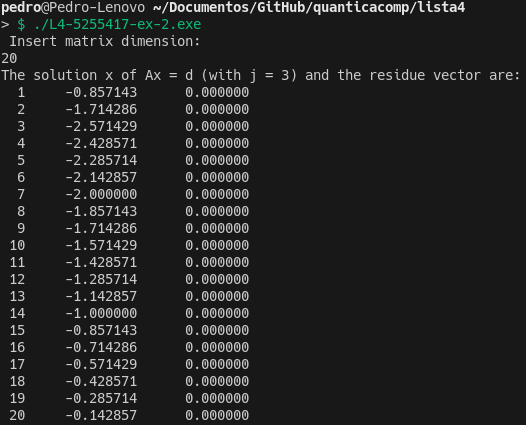
\includegraphics[width=0.8\textwidth]{../images/ex2-results-20.png}
            }
            \hfill
            \subfloat[]{
                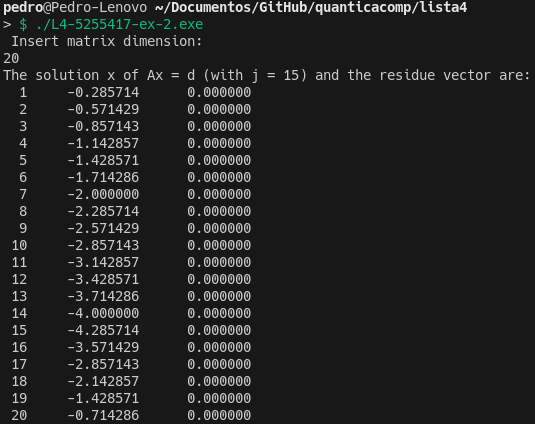
\includegraphics[width=0.8\textwidth]{../images/ex2-results-20-2.png}
            }
            \caption{Teste para matriz de dimensão 20}
        \end{figure}

        Como todos os vetores res\'iduo obtidos foram nulos, sabemos que o c\'odigo funciona de acordo com o esperado - obtendo o autovetor x corretamente.
        
\end{document}